\section{Eksperymenty}
Wykonaliśmy szereg testów, sprawdzających jak działa aplikacja w zależności od następujących parametrów:
\begin{itemize}
    \item liczebność populacji
    \item liczebność populacji $\mu$
    \item liczba prostokątów w osobniku
    \item strategia krzyżowania
    \item strategia wybierania kolejnej generacji populacji
\end{itemize}

\subsection{Eksperymenty i wyniki}
W celu uzyskania możliwie jak najbardziej prawdziwych wyników dla każdego przypadku testowego, każdy eksperyment z danymi parametrami był przeprowadzony 5 razy. Wszystkie testy zostały wykonane dla obrazu na Rysunku~\ref{fig:test_image} oraz dla z warunkami zakończenia 1000 iteracji lub dokładność 99\%. 
\begin{figure}[H]
    \centering 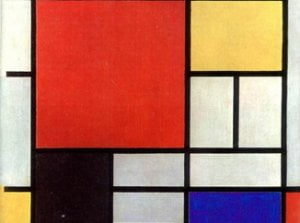
\includegraphics[width=0.5\linewidth]{img/simple_img.jpg}
    \caption{Obrazek użyty w ekseprymentach}
    \label{fig:test_image}
\end{figure}
Gdy nie było to przedmiotem eksperymentu to metodą krzyżowania było uśrednianie, a metodą wybierania - wybór najlepszych. Wykresy są tworzonę na podstawie punktów w których zmieniała się wartość funkcji dopasowania dla najlepszego osbnika, dlatego niektóre przebiegi kończą się wcześniej. Oznacza to, że wynik się nie zmienił już do końca eksperymentu.

\subsection*{Wpływ liczebności populacji}
Test wpływu liczebności populacji został przeprowadzony dla populacji o wielkościach: 2, 10, 15, 30, 40, 50, 100, liczbie prostokątów w osobniku równej 20, wielkości populacji $\mu$ będącej 1,5 raza większej od wielkości testowanej populacji.

\subsection*{Wpływ liczebności populacji $\mu$}
Test wpływu liczebności populacji $\mu$ został przeprowadzony dla stałej wielkości populacji $\lambda$ równej 40 na podstawie której kolejne przypadki testowe był obliczane za pomocą wartości procentowych: 110\%(44), 130\%(52),
150\%(60), 200\%(80), 250\%(100), 300\%(120). Liczba prostokątów w osobniku była równa 20.

\subsection*{Wpływ liczby prostokątów w osobniku}
Następny test został przeprowadzony dla następujących liczb prostokątów w osobniku: 10, 20, 50, 100, 200, 300. Wielkość populacji wynosiła 10, podpopulacji 15. Pozostałe parametry zostały niezmienione względem poprzedniego testu. 

\subsection*{Wpływ użytej strategii krzyżowania}
Dla populacji $\lambda$ - 20, populacji $\mu$ - 30 i liczbie 20 prostokątów w osobniku testy zostały przeprowadzone dla uśredniania i interpolacji.

\begin{figure}[h!]
    \centering 
    \begin{subfigure}[b]{0.49\linewidth}
        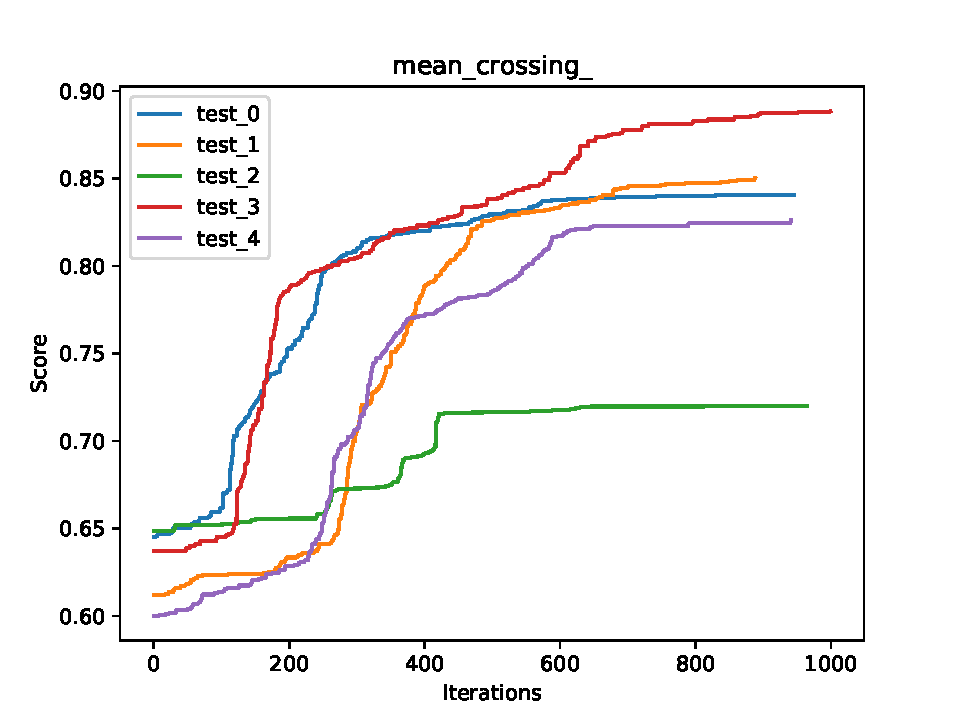
\includegraphics[width=\linewidth]{img/mean_crossing_.pdf}
        \caption{Uśrednianie}
    \end{subfigure}
    \begin{subfigure}[b]{0.49\linewidth}
        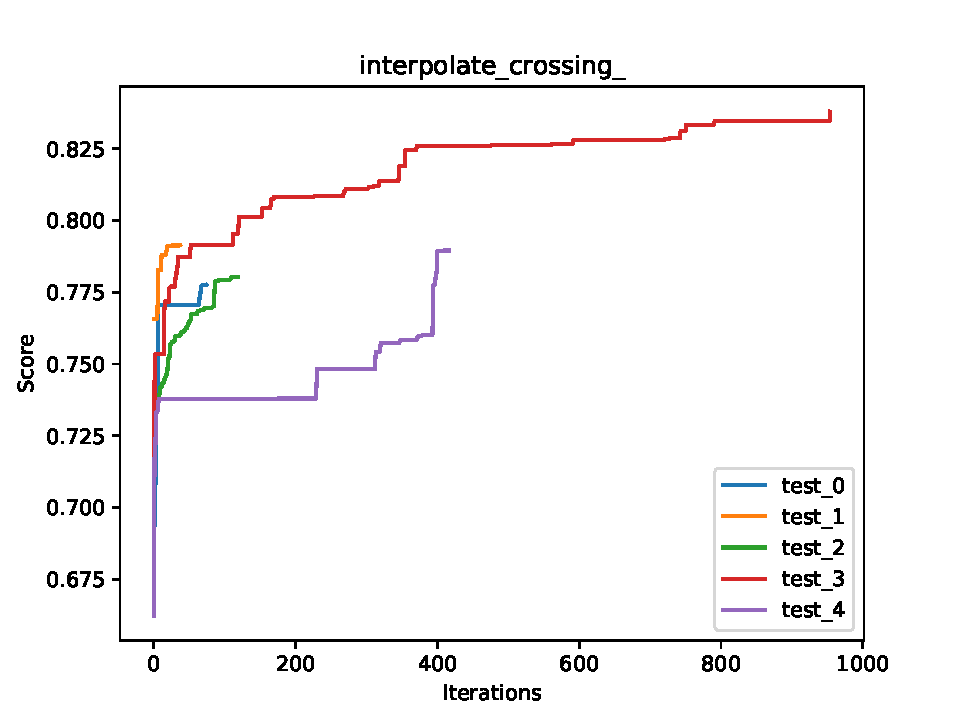
\includegraphics[width=\linewidth]{img/interpolate_crossing_.pdf}
        \caption{Interpolacja}
    \end{subfigure}
    \caption{Krzyżowanie}
    \label{fig:crossing}
\end{figure}

\begin{table}[H]
    \centering
    \begin{tabular}{|c|c|c|}
    \hline
    Metoda       & Najlepszy osobnik & Średnio najlepszy osobnik \\ \hline
    Uśrednianie  & 89\%              & 83\%                      \\ \hline
    Interpolacja & 83\%              & 79\%                      \\ \hline
    \end{tabular}
    \caption{Wyniki testów krzyżowania}
    \label{tab:crossing}
\end{table}

Dość dobrze widać, że w przypadku naszego problemu lepiej się sprawdza uśrednianie. Jeśli chodzi o interpolacje to warto zauważyć że wartości rosną bardzo szybko na początku, a potem zwykle zostają stałe lub niewiele się zmieniają. Może to być spowodowane, że algorytm dość szybko znajduje w naszym przypdaku osobnika z jednym lub kilkoma dużymi kwadrawtami, które potem ciężko rozmnożyć na lepsze osbniki. W przypadku uśredniania osbniki zmieniają się znacznie wolniej i taka sytuacja zachodzi rzadziej. 

\subsection*{Wpływ użytej strategii wybierania kolejnej populacji}
Dla populacji $\lambda$ - 20, populacji $\mu$ - 30 i liczbie 20 prostokątów w osobniku testy zostały przeprowadzone dla wyboru najlepszych, ruletki i metody rankingu.

\begin{figure}[h!]
    \centering 
    \begin{subfigure}[b]{0.49\linewidth}
        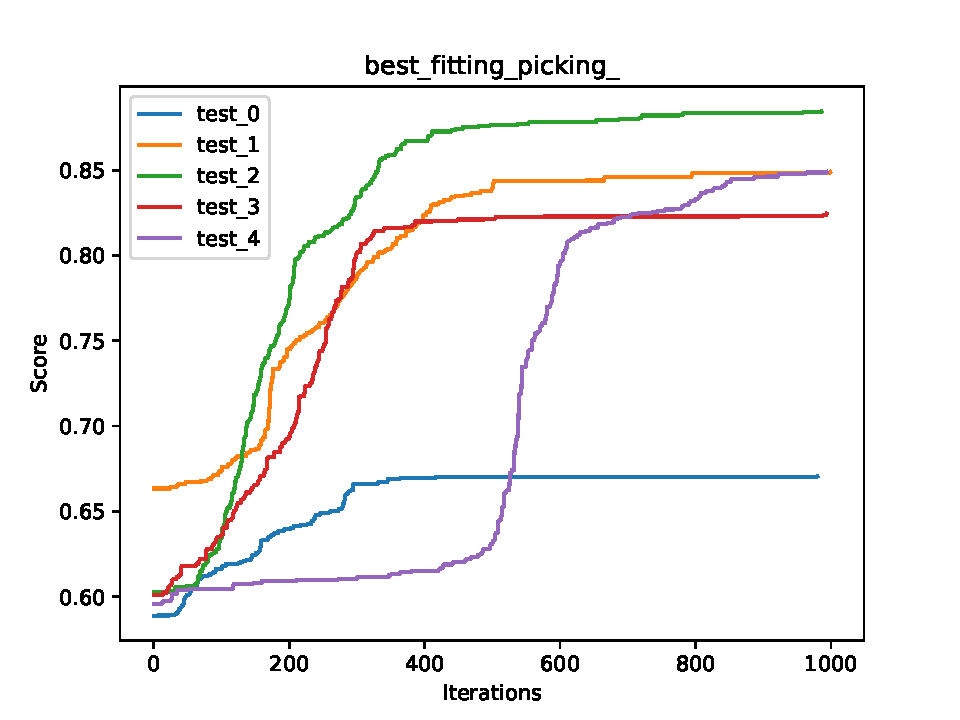
\includegraphics[width=\linewidth]{img/best_fitting_picking_.pdf}
        \caption{Wybór najlepszych}
    \end{subfigure}
    \begin{subfigure}[b]{0.49\linewidth}
        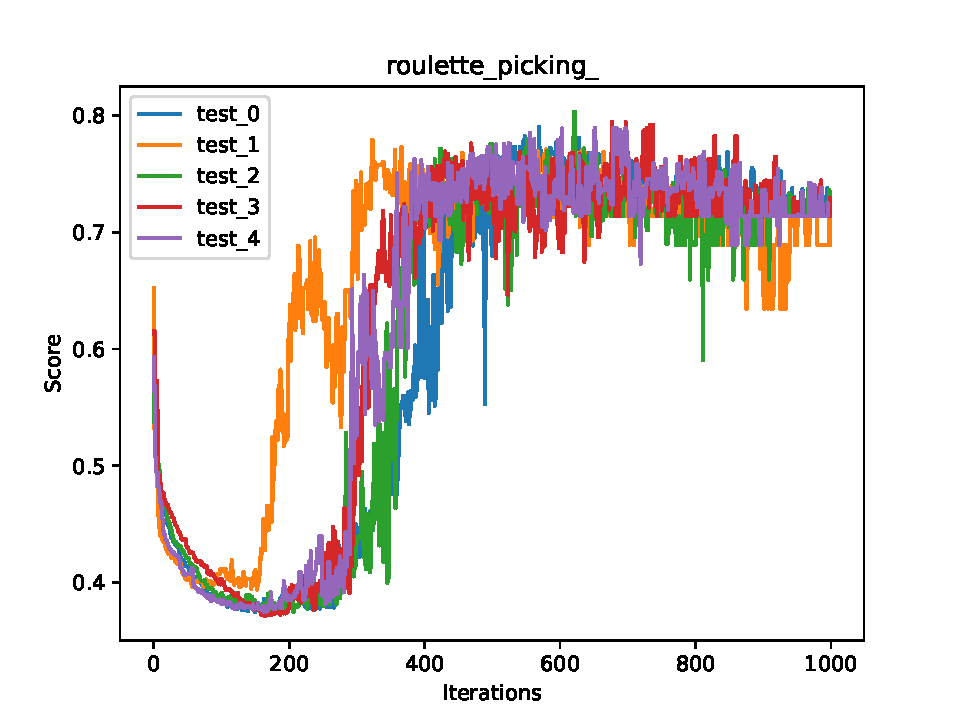
\includegraphics[width=\linewidth]{img/roulette_picking_.pdf}
        \caption{Ruletka}
    \end{subfigure}
    \begin{subfigure}[b]{0.49\linewidth}
        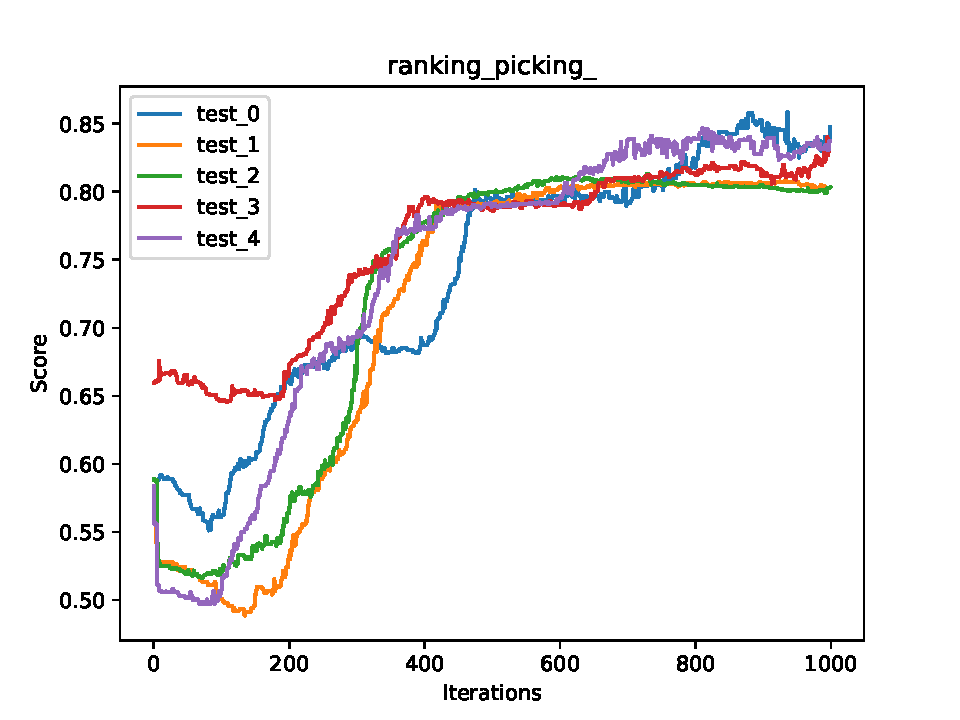
\includegraphics[width=\linewidth]{img/ranking_picking_.pdf}
        \caption{Ranking}
    \end{subfigure}
    \caption{Wybieranie}
    \label{fig:picking}
\end{figure}

\begin{table}[H]
    \centering
    \begin{tabular}{|c|c|c|}
    \hline
    Metoda       & Najlepszy osobnik & Średnio najlepszy osobnik \\ \hline
    Wybór najlepszych  & 88\%              & 82\%                      \\ \hline
    Ruletka      & 73\%              & 72\%                      \\ \hline
    Ranking      & 85\%              & 82\%                      \\ \hline
    \end{tabular}
    \caption{Wyniki testów wybierania}
    \label{tab:picking}
\end{table}
Ciężko stwierdzić, która metoda wybierania jest najlepsza, ale skłaniamy się do preferęcji wyboru najlepszych lub przez ranking. Metoda ruletki wydaje się produkować najsłabsze rezultaty. Metoda wyboru najlepszych w późniejszych fazach traci mocno na efektywności. Metoda rankingu również w późniejszej fazie nieco zwalnia ale nie tak bardzo i wydaje się być dobrym rozwiązaniem dla naszego problemu.
\subsection{Wnioski}